\documentclass[]{standalone}

\begin{document}
	\begin{frame}{Data Set}{Head MRI Scans}
	\vspace{-25pt}
	\begin{columns}
		\begin{column}{0.5\textwidth}
		\begin{exampleblock}{}
		\begin{itemize}
		\small
			\item 57 MRI \textbf{T1W} and \textbf{FLAIR} head scans;
			\item Acquired from 2009 to 2020;
			\item From three different medical centers in italy;
			\item High \textbf{heterogeneity} in acquisition parameters;
			\item Mainly \textbf{underaged} patients;
			\item Manual SCIs segmentation for each scan.
		\end{itemize}
		\end{exampleblock}
		\end{column}
		\begin{column}{0.52\textwidth}
		\vspace{-5pt}
		\begin{figure}[h!]
			\centering
			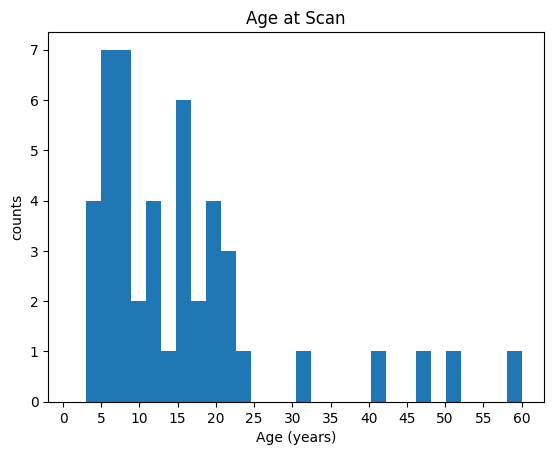
\includegraphics[scale = 0.3]{./IMG/Age.png}
		\end{figure}
		\vspace{-15pt}
		\begin{figure}[h!]
			\centering
			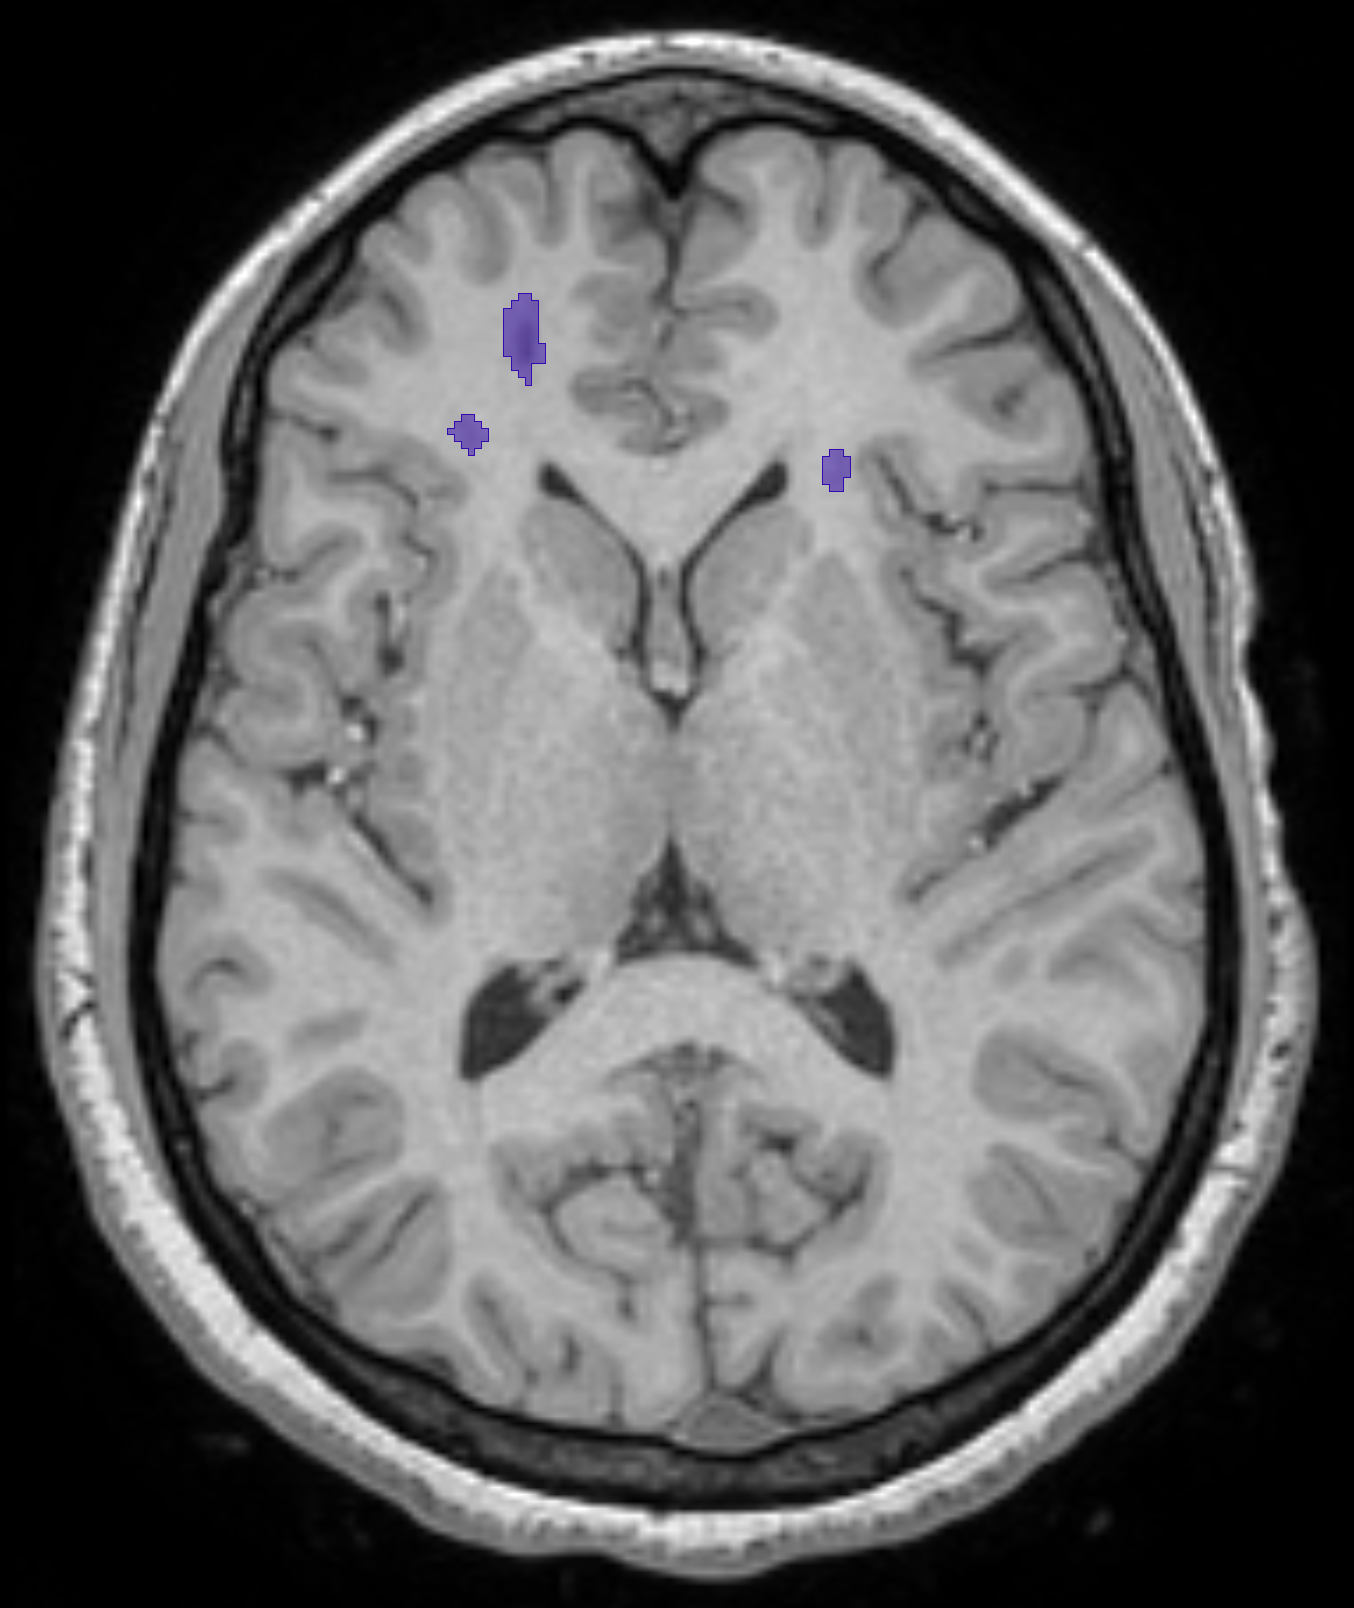
\includegraphics[scale = 0.06]{./IMG/gnd_labels.png}
		\end{figure}
		
		
		\end{column}
	\end{columns}
	\end{frame}
\end{document}
